\documentclass[%
 sor,
%aip,
%twoside,
%groupedaddress,
%jmp,
 jor,
 amsmath,amssymb,
%preprint,%
 reprint,%
%author-year,%
%author-numerical,%
]{revtex4-2}


\usepackage{natbib}
\usepackage{graphicx}% Include figure files
\usepackage{xcolor}
\usepackage{circuitikz}
\usepackage{siunitx}
\usepackage{dcolumn}% Align table columns on decimal point
\usepackage{bm}% bold math
\usepackage{amsmath, amssymb, amsfonts}
\usepackage{placeins}
\usepackage{float}
\usepackage{gensymb}
\usepackage{array}
\usepackage{siunitx}
\usepackage{enumitem}

\graphicspath{ {./images/} }

\begin{document}

\preprint{IDK what this does}

\title{Experiment 5\\Photoelectric Effect}

\author{Aumshree P. Shah\\20231059\color{red}}
\altaffiliation[\color{red}]{aumshree.pinkalbenshah@students.iiserpune.ac.in}
\date{\today}
\vspace{1cm}
\begin{abstract}
\centering
In this experiment, we attempt to measure Planck's constant and test the validity of the inverse square law.
\end{abstract}
\maketitle
\section{Theory and Procedure}
\subsection{Theory}
It was observed as early as 1905 that most metals under influence of radiation, emit electrons. This phenomenon was termed as photoelectric emission. The detailed study of it has shown:
\begin{enumerate}
  \item That the emission process depends strongly on frequency of radiation.
  \item For each metal there exists a critical frequency such that light of lower frequency is unable to liberate member of electrons is strictly proportional to the intensity of this radiation.
  \item The emission of electron occurs within a very short time interval after arrival of the radiation and member of electrons is strictly proportional to the intensity of this radiation. 
\end{enumerate}
The experimental facts given above are among the strongest evidence that the electromagnetic field is quantified and the field consists of quanta of energy $E = h \nu$ where $\nu$ is the frequency of the radiation and $h$ is the Planck’s constant. These quanta are called photons. \\

Further it is assumed that electrons are bound inside the metal surface with an energy $e\phi$, where $\phi$ is called work function. It then follows that if the frequency of the light is such that $h\nu > e \phi$ it will be possible to eject photoelectron, while if $h\nu < e \phi$, it would be impossible. In the former case, the excess energy of quantum appears as kinetic energy of the electron, so that \begin{equation}h\nu = \frac 1 2 mv^2 + e\phi \end{equation} which is the famous photoelectrons equation formulated by Einstein in 1905. The energy of emitted photoelectrons can be measured by simple retarding potential techniques as is done in this experiment.
Retarding potential at which the photocurrent stopped, we call it stopping potential ($V_s$) and it's used to measure the kinetic energy of photoelectrons ($E_e$), we have: 
\begin{equation}E_e = \frac 1 2 mv^2 = eV_s \,\,\,\,\,\,\,\,\,\,\,\,\,\,  \text{or} \,\,\,\,\,\,\,\,\,\,\,\,\,\, V_s = \frac h e \nu-\phi \end{equation}
So when we plot the graph of $V_s$ as a function of $\nu$, the slope has a value of $\frac h e $ and it intercepts on x-axis at $V_s = 0$ and the $\nu$ at the intercept with the slope of the graph gives the work function $\phi$.


\subsection{Procedure}

\begin{enumerate}
	\item Read the user manual of the setup (Refer to Refernce-\cite{fsu_manual}).
  \item Insert the red color filter (635 nm), set light intensity switch at strong light, voltage direction switch at `-', display mode switch at current display.
  \item Adjust to de-accelerating voltage to 0 $V$  and set current range selector at X 0.001. Increase the de-accelerating to decrease the photo current to zero. Take down the de-accelerating voltage $(V_s)$ corresponding to zero current of 635 nm wavelength. Get the $V_s$ of other wave lengths, in the same way.
  \item For verification of inverse square law, remove filters, fix the intensity of light around a proper value, and take the current values by varing the light source at different distance from the vaccum-tube.
\end{enumerate}


\subsection{Precautions}
\begin{itemize}
  \item Ensure there is no obstruction between the source and the photo-tube (see Appendix~\ref{appendix:prevexp}).
  \item Clean all the filters properly
   \item Check weather the filters work   (see Appendix~\ref{appendix:filters}).
\end{itemize}




\section{Observations}


\begin{table}[ht]
\centering
    \begin{minipage}[b]{0.48\hsize}\centering
\begin{tabular}{|c|c|c|}
\hline
\textbf{Filter}& \textbf{No. of } & \textbf{Voltage} \\
\textbf{Wavelength (nm)} & \textbf{filters}& \textbf{(V)}		\\
\hline
635 & 1 &	-0.32		\\
585 & 4 &	 -0.48        \\  
540 & 3 &	  -0.65       \\
500 & 4 &	   -0.71      \\
460 & 2 &	    -0.99     \\

\hline
\end{tabular}
\caption{Stopping voltage at different filters, with source at $l=25.0 \si{\centi\meter}$. Data taken on 11-Mar-2025}
\label{tab:table1}
\[
\boxed{
\begin{aligned}
         \text{Least count of Voltage}  &= 0.01\si{\volt} \\
	 \text{Least count of Current}  &= 10^{-7}~\si{\ampere} \\
	 \text{Least count of Wavelength}  &= 10^{-8}~\si{\meter} \\
\end{aligned}
}
\]


\end{minipage}
\hfill\vline\hfill
    \begin{minipage}[b]{0.48\hsize}\centering
\begin{tabular}{|c|c|}
\hline
\textbf{Distance } & \textbf{Current} \\
\textbf{(cm)} & \textbf{($\mu$A)} \\
\hline
16.0 	 &12.2 		\\
18.0 	 &10.0          \\  
20.0 	 & 7.6          \\
24.0 	 & 4.9          \\
30.0 	 & 3.3          \\
35.0 	 & 2.5  	\\
40.0 	 & 2.2  	\\
\hline
\end{tabular}
\caption{Current at different distances, fixed intensity. Data taken on 11-Mar-2025 }
\label{tab:table2}
\[ \boxed{
 \begin{aligned}
         \text{Least count of Voltage}  &= 0.01\si{\volt} \\
	 \text{Least count of Current}  &= 10^{-7}~\si{\ampere} \\
         \text{Least count of Length}  &= 0.0001~\si{\meter} \\
 \end{aligned}
}
\]

   \end{minipage}
\end{table}


\section{Uncertainties and Sources of Error}
\subsection{Uncertainties from precision of instrument}
\begin{itemize}
    \item Distance Measurements:
    All length values have an uncertainty of $\Delta l = \pm 0.5$ \si{\milli\meter} due to instrument resolution.    
\item Current Measurements: Current values have an uncertainty of $\Delta A = \pm 5\times10^{-8}$ \si{\ampere} due to instrument resolution. 
    \item Voltage Measurements: Voltage values have an uncertainty of $\Delta V = \pm 0.005$ \si{\volt} due to instrument resolution. 
    \item Filter Uncertanity: To account for the error in non-ideal filters, we take the uncertainity to be $\pm 5$ nm.
\end{itemize}

\subsection{Systematic Errors}

\section{Calculation and Error Analysis}

\subsection{Plank's constant}
To calculate the Plank's constant we use Equation-2, and plot the graph of $V_s$ vs $\nu$. The slope of the graph will have value of $h/e$. Now since $c = \lambda\nu$, this gives us $\nu = c/\lambda$ and \textbf{ENTER A BOOK REFRENCE HERE} $$\Delta \nu = c\frac{\Delta \lambda}{\lambda^2}$$

Plotting the graph of $\nu \text{ vs } V_s$ with their respective uncertanity: \textbf{ENTER A CODE REFRENCE HERE} 

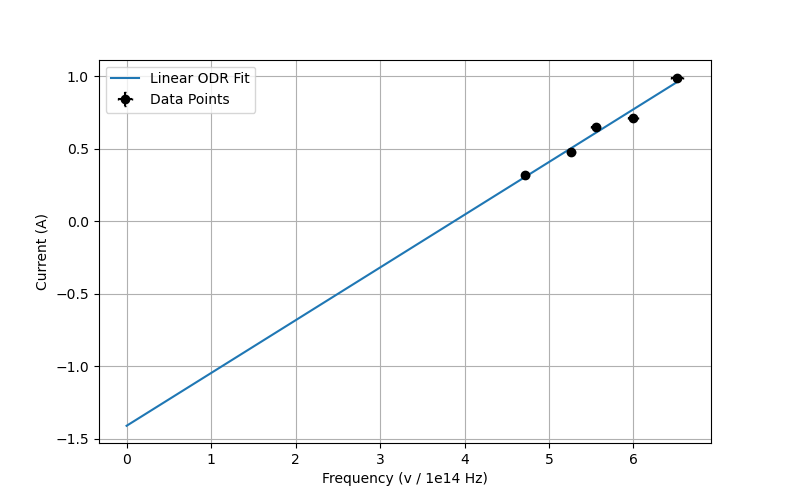
\includegraphics[scale=0.69]{image1}\\
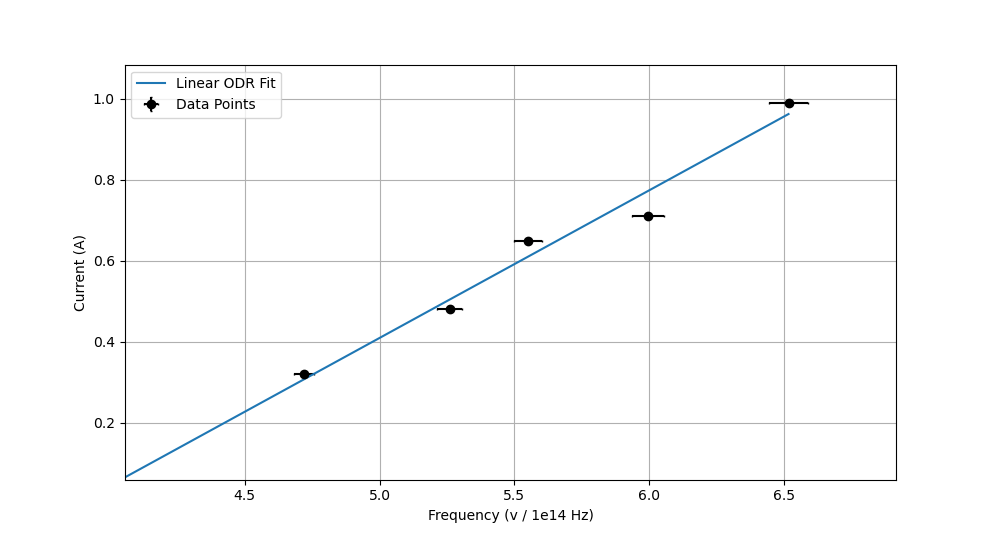
\includegraphics[scale=0.69]{image 2}

Optimized Parameters: [ 0.36404357 -1.41054501]

Parameter Errors: [0.03307623 0.17843993]




\subsection{Inverse Square Law}
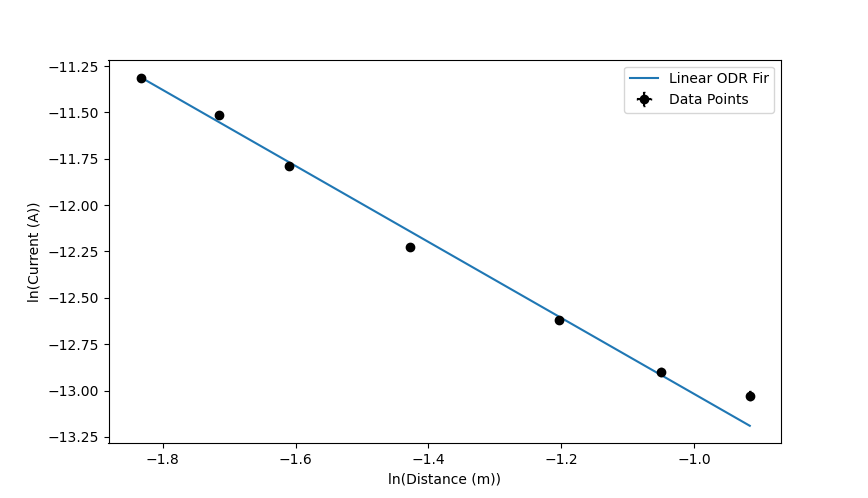
\includegraphics[scale=0.69]{image}
Optimized Parameters: [ -2.04953181 -15.06801565]
Parameter Errors: [0.08743895 0.14215498]


\section{Result}
\ref{github}

The reference resistance was determined to be: $R_0 = 2.90 \pm 7.7\% $. (This error accounts for uncertainty in temperature measurements)\\

The Stefan-Boltzmann fit for the tungsten filament showed:
$$
P = (4.00 \pm 0.066) \times 10^{-14}\ \mathrm{T^4}
$$

The log-log analysis revealed a power-law relationship:
$$
\log P = (3.98 \pm 0.06)\log T + (-30.71 \pm 0.48)
$$

\noindent\fbox{%
    \parbox{\textwidth}{%
       The measured slope of $m = 3.98 \pm 0.06$ agrees with Stefan's law prediction of $P \propto T^4$, as the theoretical value of 4 lies within the experimental uncertainty range.
       }%
}\\
\\
As observed in previous trials, the equipment malfunctioned multiple times (see Appendix~\ref{appendix:prevexp}).  

To account for filtering issues, multiple filters were used (see Appendix~\ref{appendix:filters}).  

Anomalies in voltage readings, especially with the blue filter, were noted (see Appendix~\ref{appendix:bluefilter}).

\noindent\rule{\linewidth}{0.4pt}
\vspace{2cm}


\appendix
\section{Equipment Faulty on Multiple Occasions} \label{appendix:prevexp}
This experiment was performed multiple times, but the obtained values were highly inconsistent. Later, it was discovered that the instrument contained styrofoam inside, which needed to be removed.  
\section{Filters Not Working} \label{appendix:filters}
The filters used in the experiment were not proper optical filters and, as a result, did not effectively filter light. Therefore, multiple filters were used for a given wavelength.  

\section{Blue Filter Error} \label{appendix:bluefilter}
The values obtained with the addition of the blue filter appear incorrect. Without any filter, the voltage should not exceed $0.88V$, but the blue filter resulted in a reading of $0.99V$.  





... as discussed in \cite{PrestonDietzErrorAnalysis}.
\cite{PrestonDietzErrorAnalysis}
Referencing the photoelectric effect \cite{wiki_photoelectric}. The code for the experiment can be found in the repository \cite{github_code}. The apparatus used is described in \cite{ses_apparatus}, and the detailed manual is available in \cite{fsu_manual}.




\bibliographystyle{unsrt}
\bibliography{aipsamp}


\end{document}
